\chapter{Class F Amplifier Fabrication and Test Results, Comparisons to Specs}

The final version of the amplifier was milled using the LPFK S62 in the Cal Poly anechoic chamber. One aspect that wasn't taken into account in the ADS simulation was cooling the amplifier during operation. Even when the amplifier is operating at high PAE, it must still dissipate a heat equal to the power that wasn't used to amplify the input signal. The heat dissipation calculations were done assuming the cooling would have to dissipate all of the DC bias power at the highest input power which for the final amplifier was equal to the 170 mA times the bias voltage of 40 V which is equal to 6.8 Watts. The cooling was done with a fan and heatsink mounted on top of the transistor by using the thermal resistance supplied by the manufacturer of the transistor to determine the cooling required. The fan draws 30 mA at 40 volts and was tied to the drain voltage of the amplifier and was included in the PAE measurements of the amplifier. Also to increase the thermal conduction in the final amplifier vias were added underneath the transistor to improve the heat conduction after the board layout was done in ADS. A photo of a previous version of the amplifier that did not have vias can be seen in Figure \ref{fig:old_amp}. Holes were drilled adjacent to the amplifier and copper tape was soldered from the ground pin on the top layer to the bottom layer was used to conduct the heat. The vias proved far superior in conducting heat because they were able to place directly underneath the transistor allowing the heat to be conducted to the ground plane with less thermal resistance.

\begin{figure}
  \centering
  % Requires \usepackage{graphicx}
  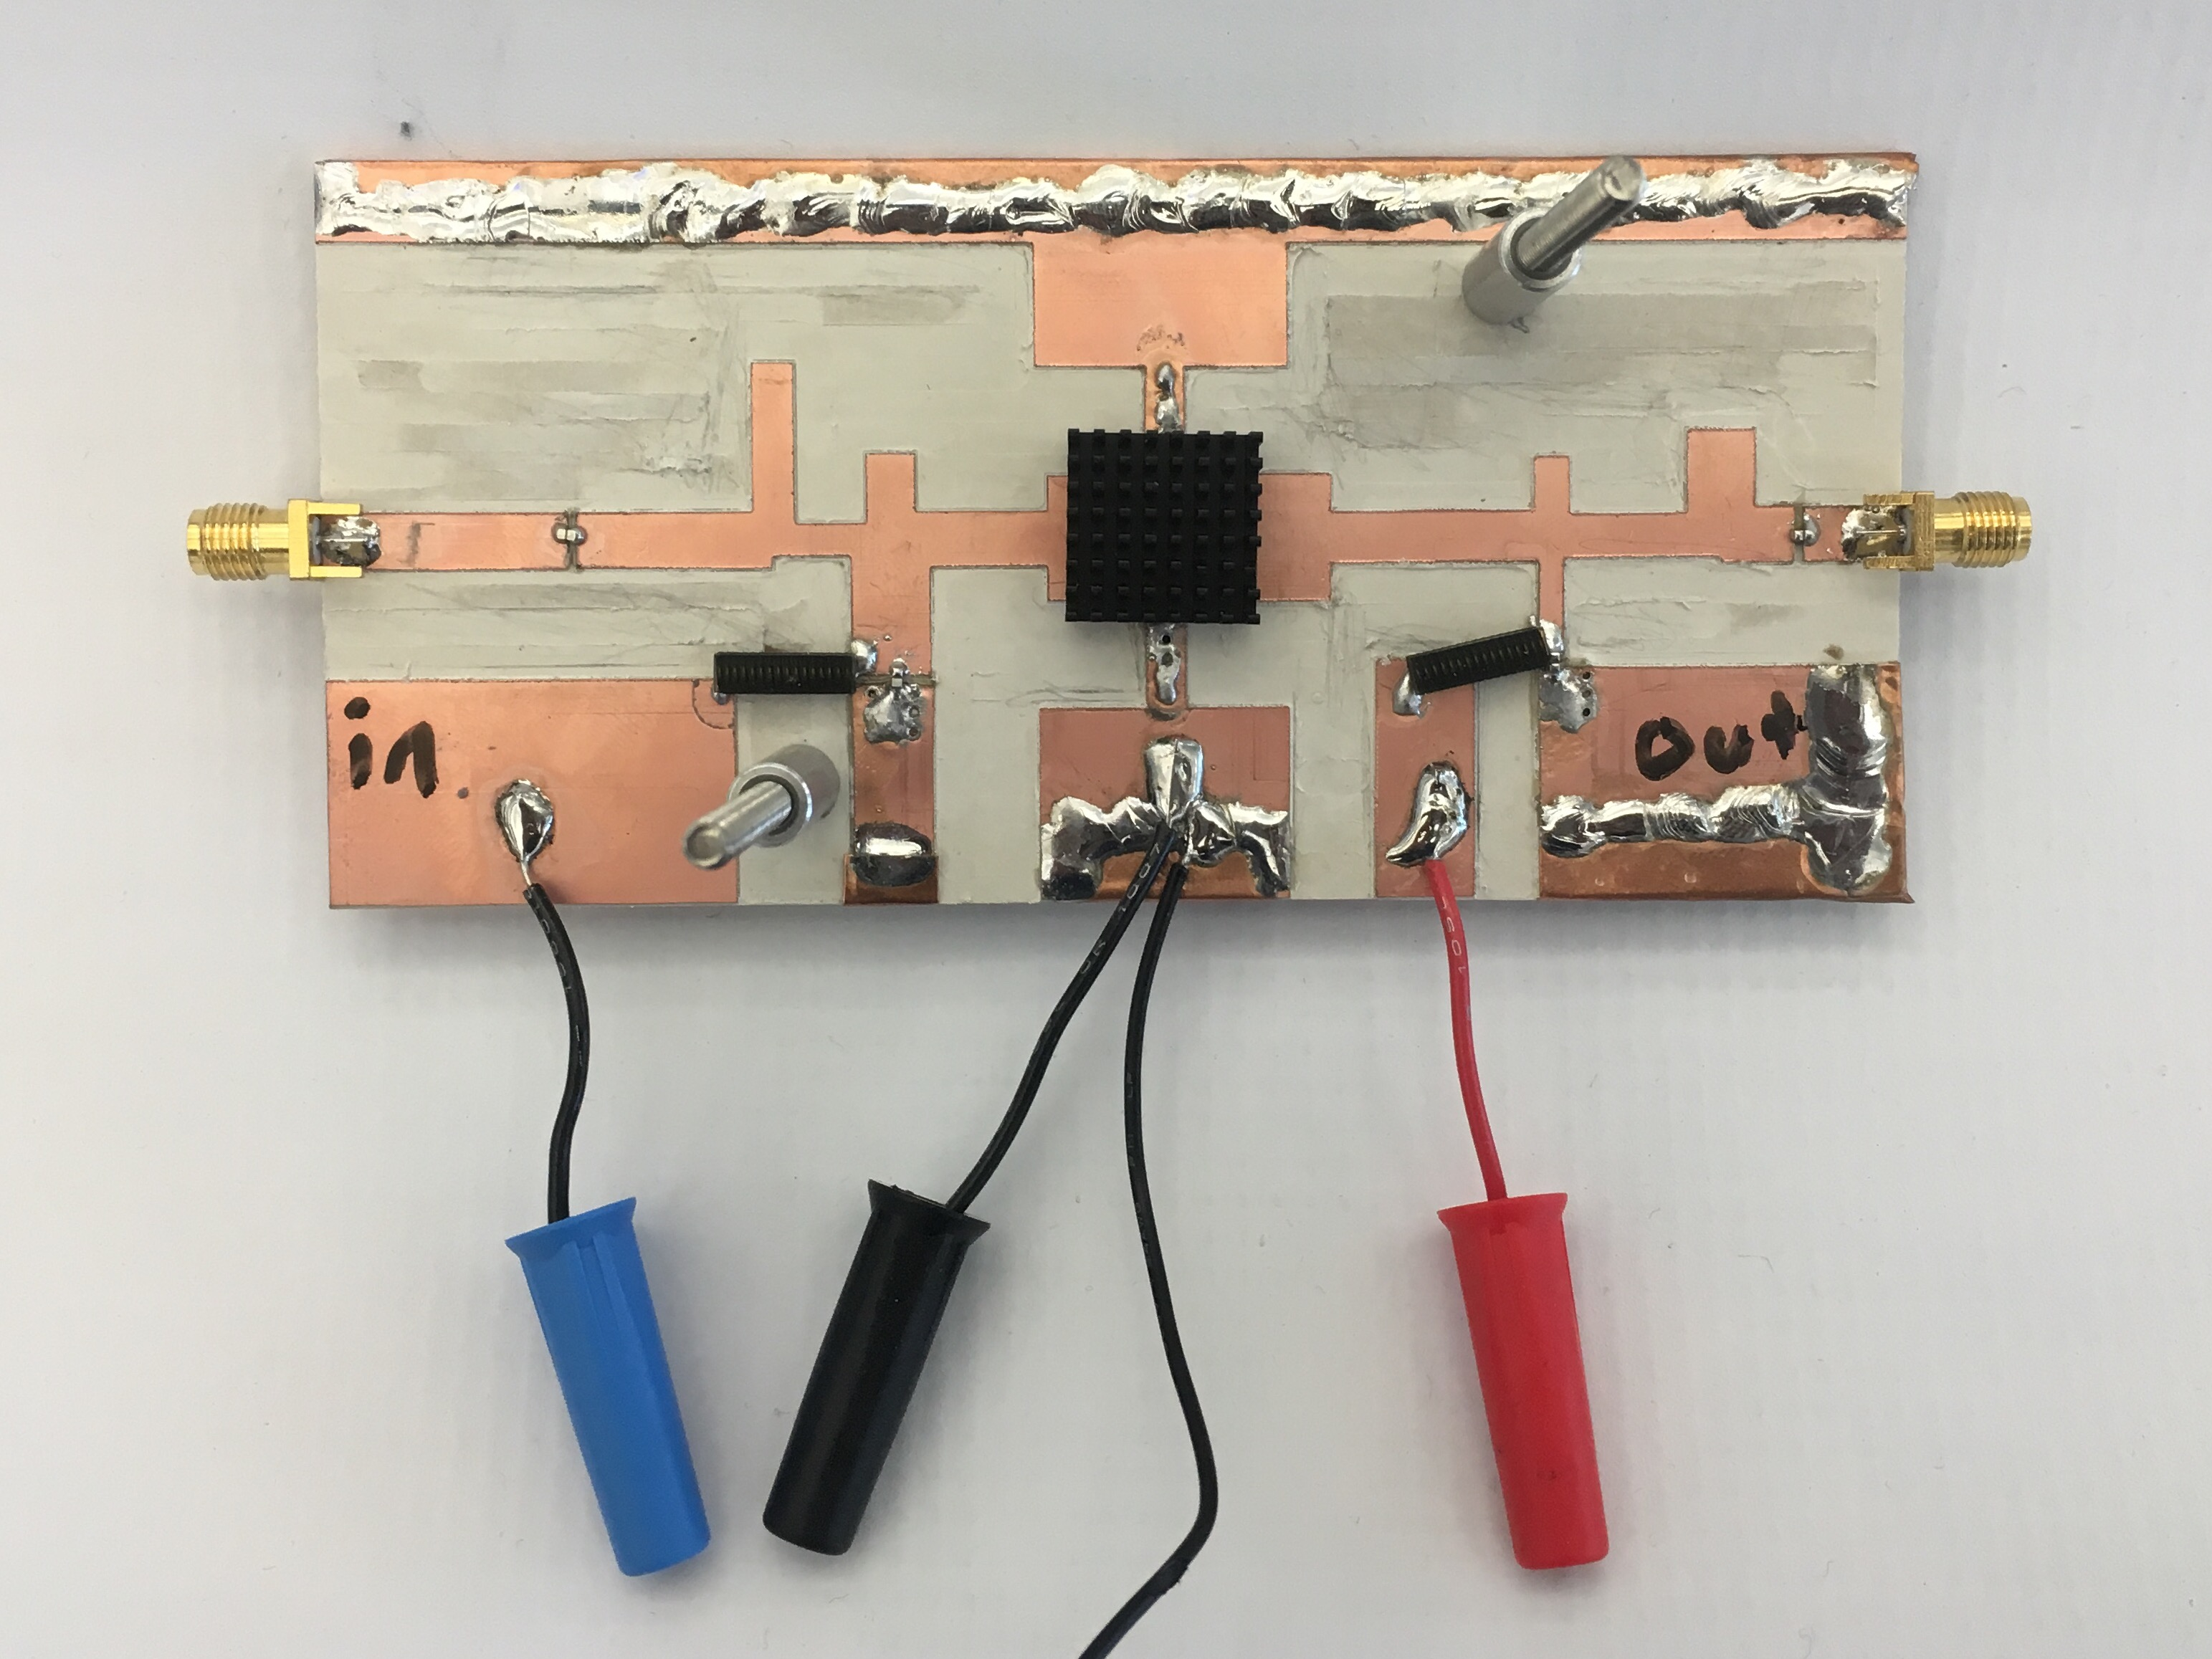
\includegraphics[width=5in,height=5in,keepaspectratio]{figures/test/final_amp}\\
  \caption{Photo of Final Amplifier Without the Fan}
  \label{fig:final_amp}

  \vspace*{\floatsep}

  \centering
  % Requires \usepackage{graphicx}
  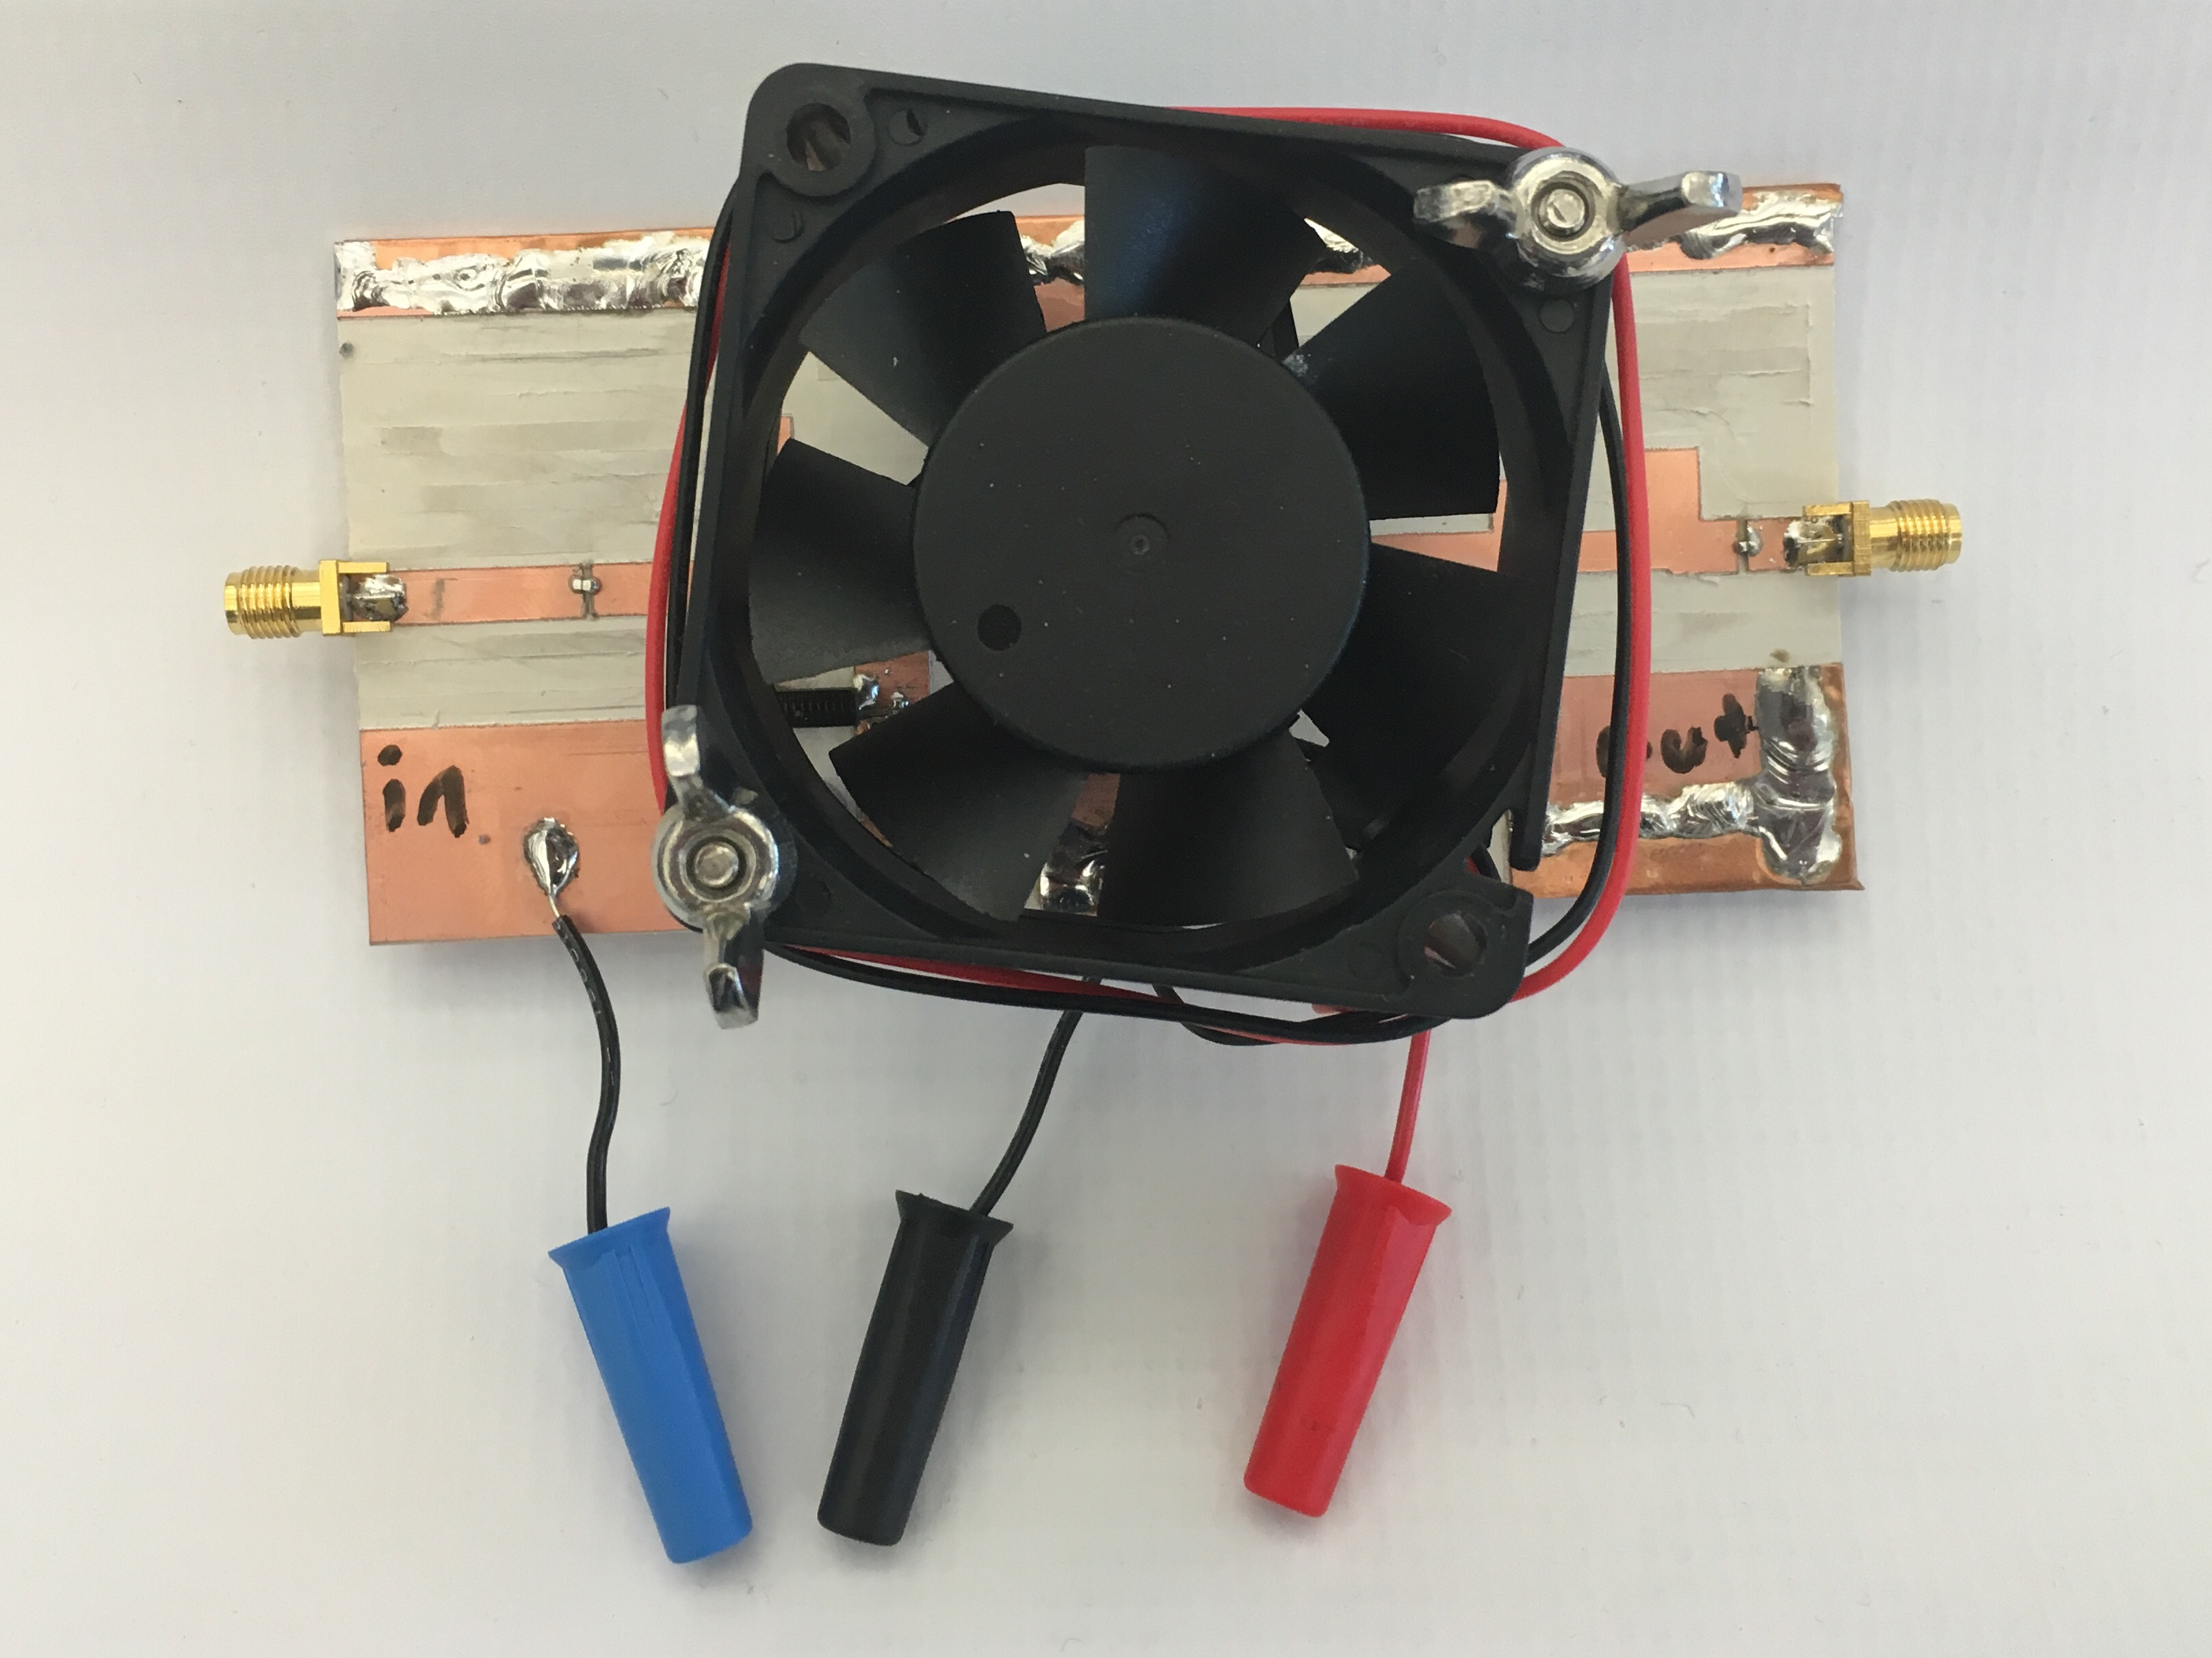
\includegraphics[width=5in,height=5in,keepaspectratio]{figures/test/final_fan}\\
  \caption{Photo of Final Amplifier With the Fan}
  \label{fig:final_fan}
\end{figure}

The bias network for the final amplifier used grounded shunt caps on the quarter wavelength stubs to create RF shorts. The DC bias was then fed through the quarter wavelength stubs through a series wideband spiral inductor. Two previous versions of the amplifier were built but due to the challenge of soldering the leadless package of the transistor they were damaged most likely due to shorts and insufficient cooling. The bias inductors, coupling capacitors, and transistor was mounted on the board using solder paste and a heatgun. SMA connectors were soldered on the input and output traces and banana plugs were soldered to the DC bias pads to comply with the competition rules. The final build of the amplifier without the fan can be seen in Figure \ref{fig:final_amp} and with the fan in Figure \ref{fig:final_fan}. The amplifier was measured with an Anritsu MS4622B and the drain powered with an Agilent Power Supply E3640A with the drain current being measured by an Agilent Multimeter Agilent U3606A. The gate voltage was powered by an Agilent Power Supply E3630A. After tuning the gate bias and measuring the amplifier performance, a final gate voltage of -2.66 V for the amplifier. A photo of the test setup can be seen in Figure \ref{fig:test_setup}.

%A bill of materials and the board layout can be found in the Appendix.

%Fix VNA part number

%A drain current versus drain-source voltage measurement at a gate voltage of -2.6 V can be seen in Figure X.

For the RF measurements the VNA was calibrated from 2 GHz to 4 GHz and set to average ten samples. A 20 dB attenuator was put at the output of the amplifier so the VNA would not be damaged by the high RF output power. The 20 dB attenuator was measured so the attenuation could be removed and the amplifier gain could be properly measured. The measured center frequency of the final amplifier was 2.91 GHz and the various measured parameters of the amplifier can be seen in Figure \ref{fig:meas_singlesweep}. The VNA used to measure the amplifier was only able output a maximum of 20 dBm of power compared to the competition maximum of 24 dBm input power which limits the maximum PAE the amplifier can achieve.

\begin{figure}
  \centering

  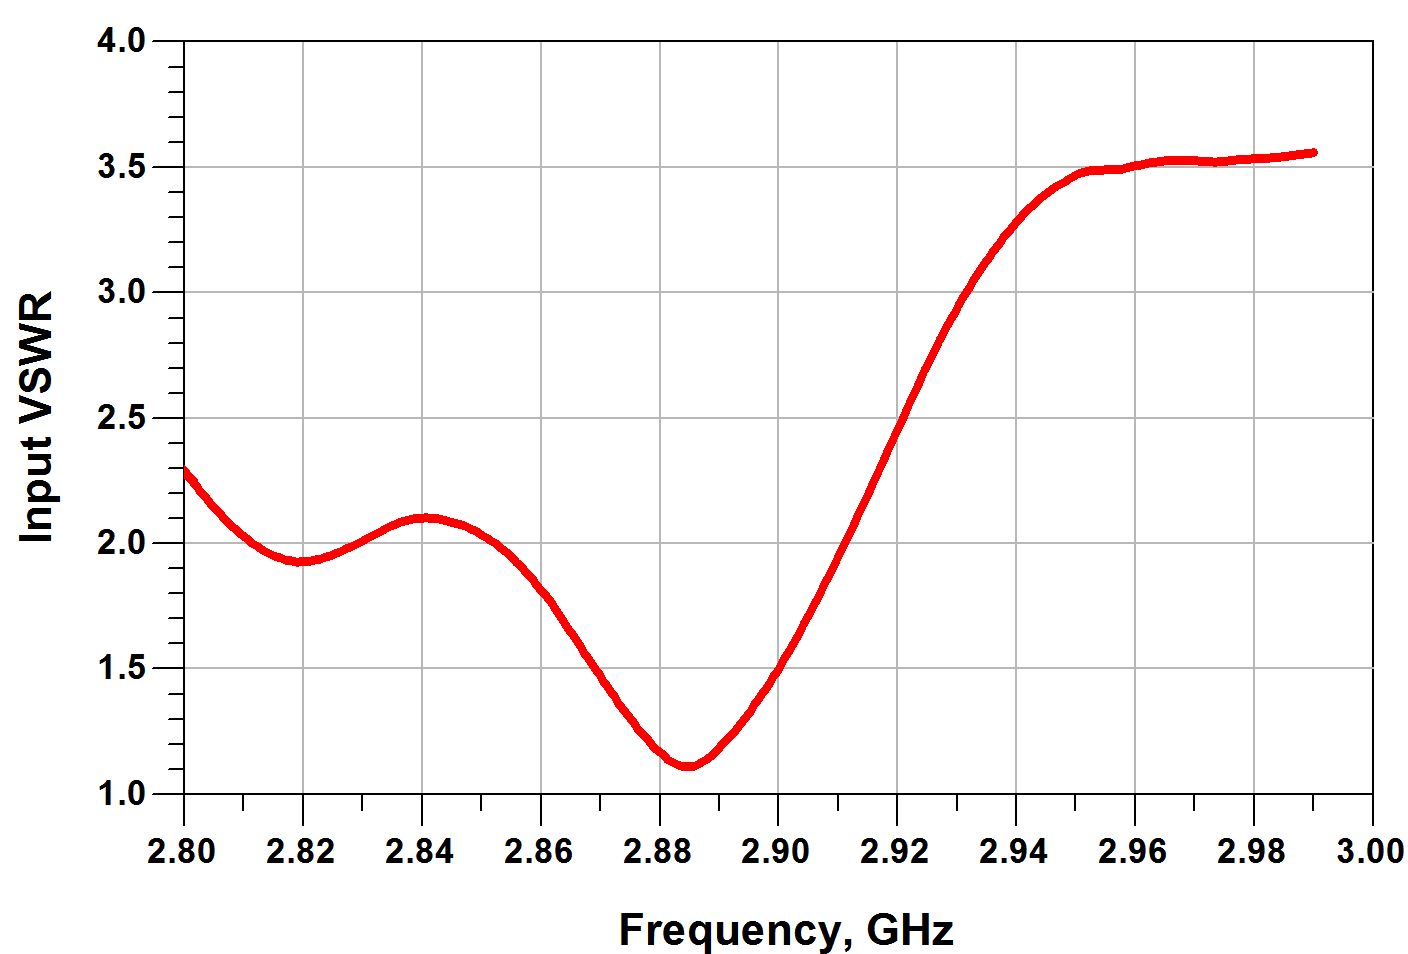
\includegraphics[width=5in,height=5in,keepaspectratio]{figures/test/input_vswr}\\
  \caption{Measured Input VSWR of Final Amplifier}
  \label{fig:input_vswr}
\end{figure}

 The amplifier s-parameters and drain current was measured over a wide range of input powers from -30 dBm to 20 dBm. Only the input VSWR seen in Figure \ref{fig:input_vswr} could be measured properly. The 20 dB attenuator at the output resulted in erroneous output VSWR when de-embedded which is most likely due to the reflection from the attenuator being larger than the reflection from the output of the amplifier. The amplifier had the best input match at slightly below the center frequency at 2.89 GHz with a VWSR of 1.11 and at the center frequency of 2.91 GHz the VSWR was measured to be 1.9.

 \begin{figure}
  \centering
  % Requires \usepackage{graphicx}
  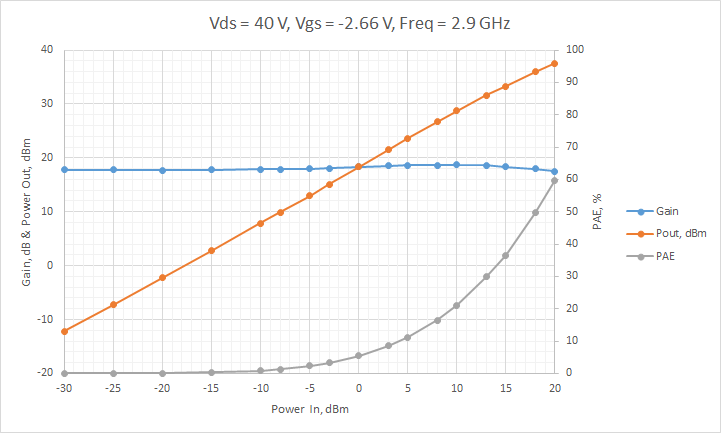
\includegraphics[width=5in,height=5in,keepaspectratio]{figures/test/meas_singletone}\\
  \caption{Measured Parameters of Final Amplifier}
  \label{fig:meas_singlesweep}

\end{figure}

 The final amplifier was able to output a maximum of 37 dBm at an input power of 20 dBm and a PAE of 59.8\% resulting in a figure of merit of 78. The amplifier is able to output 36 dBm at input powers 18 dBm or greater which is 3 dB more than the design goal. The amplifier most likely has a maximum PAE in the 70\% range at the maximum allowed input power of 24 dBm from looking at the increase in input power from 15 dBm to 20 dBM, the PAE increases from 36\% to 60\%. The amplifier has 19 dB of gain from -30 dBm to 15 dBm of input power and shows gain compression beyond 15 dBm seen in Figure \ref{fig:meas_singlesweep}.

 To qualify for the IMS competition the amplifier carrier-to-interference (C/I) ratio must be greater than 30 dB using two 5 MHz spaced tones at an input power of 0 dBm. The C/I was measured by taking an intermodulation distortion measurement of the amplifier from 2.8 GHz to 3 GHz seen in Figure \ref{fig:meas_imd}. The IMD was well below the required 30 dB and was around -80 dB across the entire frequency band. The output third order intercept (OIP3) was calculated using the IMD measurement, and can be shown in Figure \ref{fig:output_ip3}. At the center frequency of 2.9 GHz the OIP3 is around 55 dBm.

 A comparison of the amplifier measurements and the design specifications can be seen in Table \ref{table:meas_spec_compare}. It should be reiterated that it was expected the fabricated amplifier would require a higher input power than the design specification to take in account non-idealities that could not be taken into account in the simulation. The amplifier has a lower center frequency than expected but at a fixed PAE it amounts to less than a one point difference in the figure of merit. Overall while the amplifier may not have met all of the design specifications, it is still a functional class F amplifier that can compete in the design competition.

 %Table comparing the final design specs to the measurements
\begin{table}
    \centering
    \caption{Comparison of the Specification and Measured Performance of Amplifier}
    \label{table:meas_spec_compare}
    \begin{tabular}{|l|l|l|}
      \hline
      % after \\: \hline or \cline{col1-col2} \cline{col3-col4} ...
      {Parameter}                      & {Specification }   & {Measured} \\ \hline
      {Center Frequency, GHz}          & 3                  & 2.9 \\ \hline
      {Input Power for Max PAE, dBm}    & 15                 & 20 \\ \hline
      {Output Power for Max PAE, dBm}  & {\textgreater 36}  & {37} \\ \hline
      {Maximum PAE, \%}                & 70                 & {59.8} \\ \hline
      {Input and Output VSWR}          & {\textless 2}      & {\textless 2} \\ \hline
    \end{tabular}
\end{table}

 \begin{figure}
  \centering
  % Requires \usepackage{graphicx}
  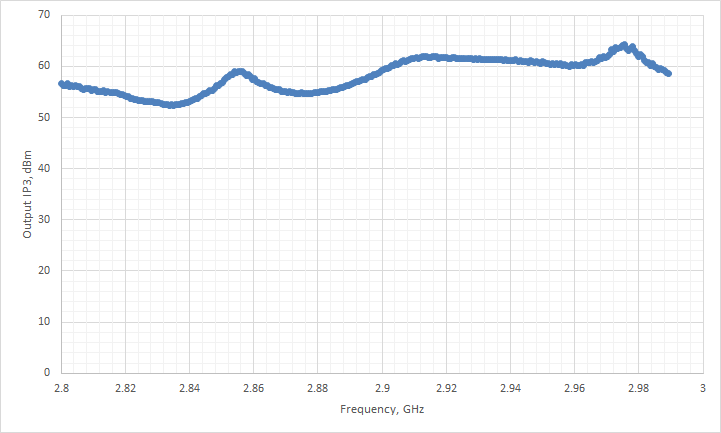
\includegraphics[width=5in,height=5in,keepaspectratio]{figures/test/output_ip3}\\
  \caption{Measured Output Third Order Intercept of Final Amplifier}
  \label{fig:output_ip3}
\end{figure}

\begin{figure}

  \centering
  % Requires \usepackage{graphicx}
  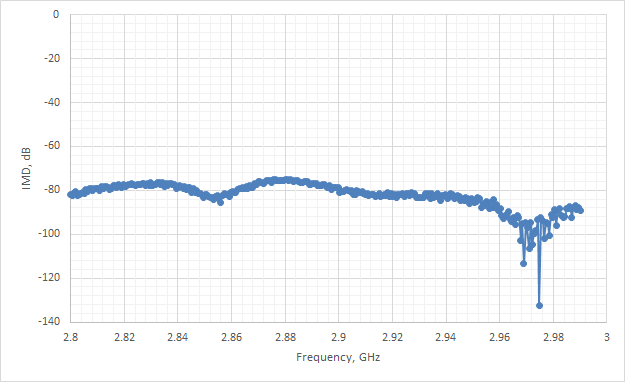
\includegraphics[width=5in,height=5in,keepaspectratio]{figures/test/meas_imd}\\
  \caption{Measured Intermodulation Distortion of Amplifier Using 2 Tones 5 MHz Apart}
  \label{fig:meas_imd}
\end{figure}

A major challenge of the thesis was finding equipment to measure the amplifier. Only one of the signal generators in the microwave laboratory was able to output 24 dBm at 3 GHz. Some of the equipment that was rated to output the RF power needed to measure the amplifier was measured on signal analyzers to be much less. No equipment was able to do the two tone test at a high power and will have to be done at the conference. The two-tone intermodulation distortion measurement had to be done on the Antritsu MS4622B VNAs which had a maximum output power of 7 dBm. Fortunately to qualify for the competition, the carrier-to-interference (C/I) specification of greater than 30 dB at 0 dBm input power was able to be measured.

\begin{figure}
  \centering
  % Requires \usepackage{graphicx}
  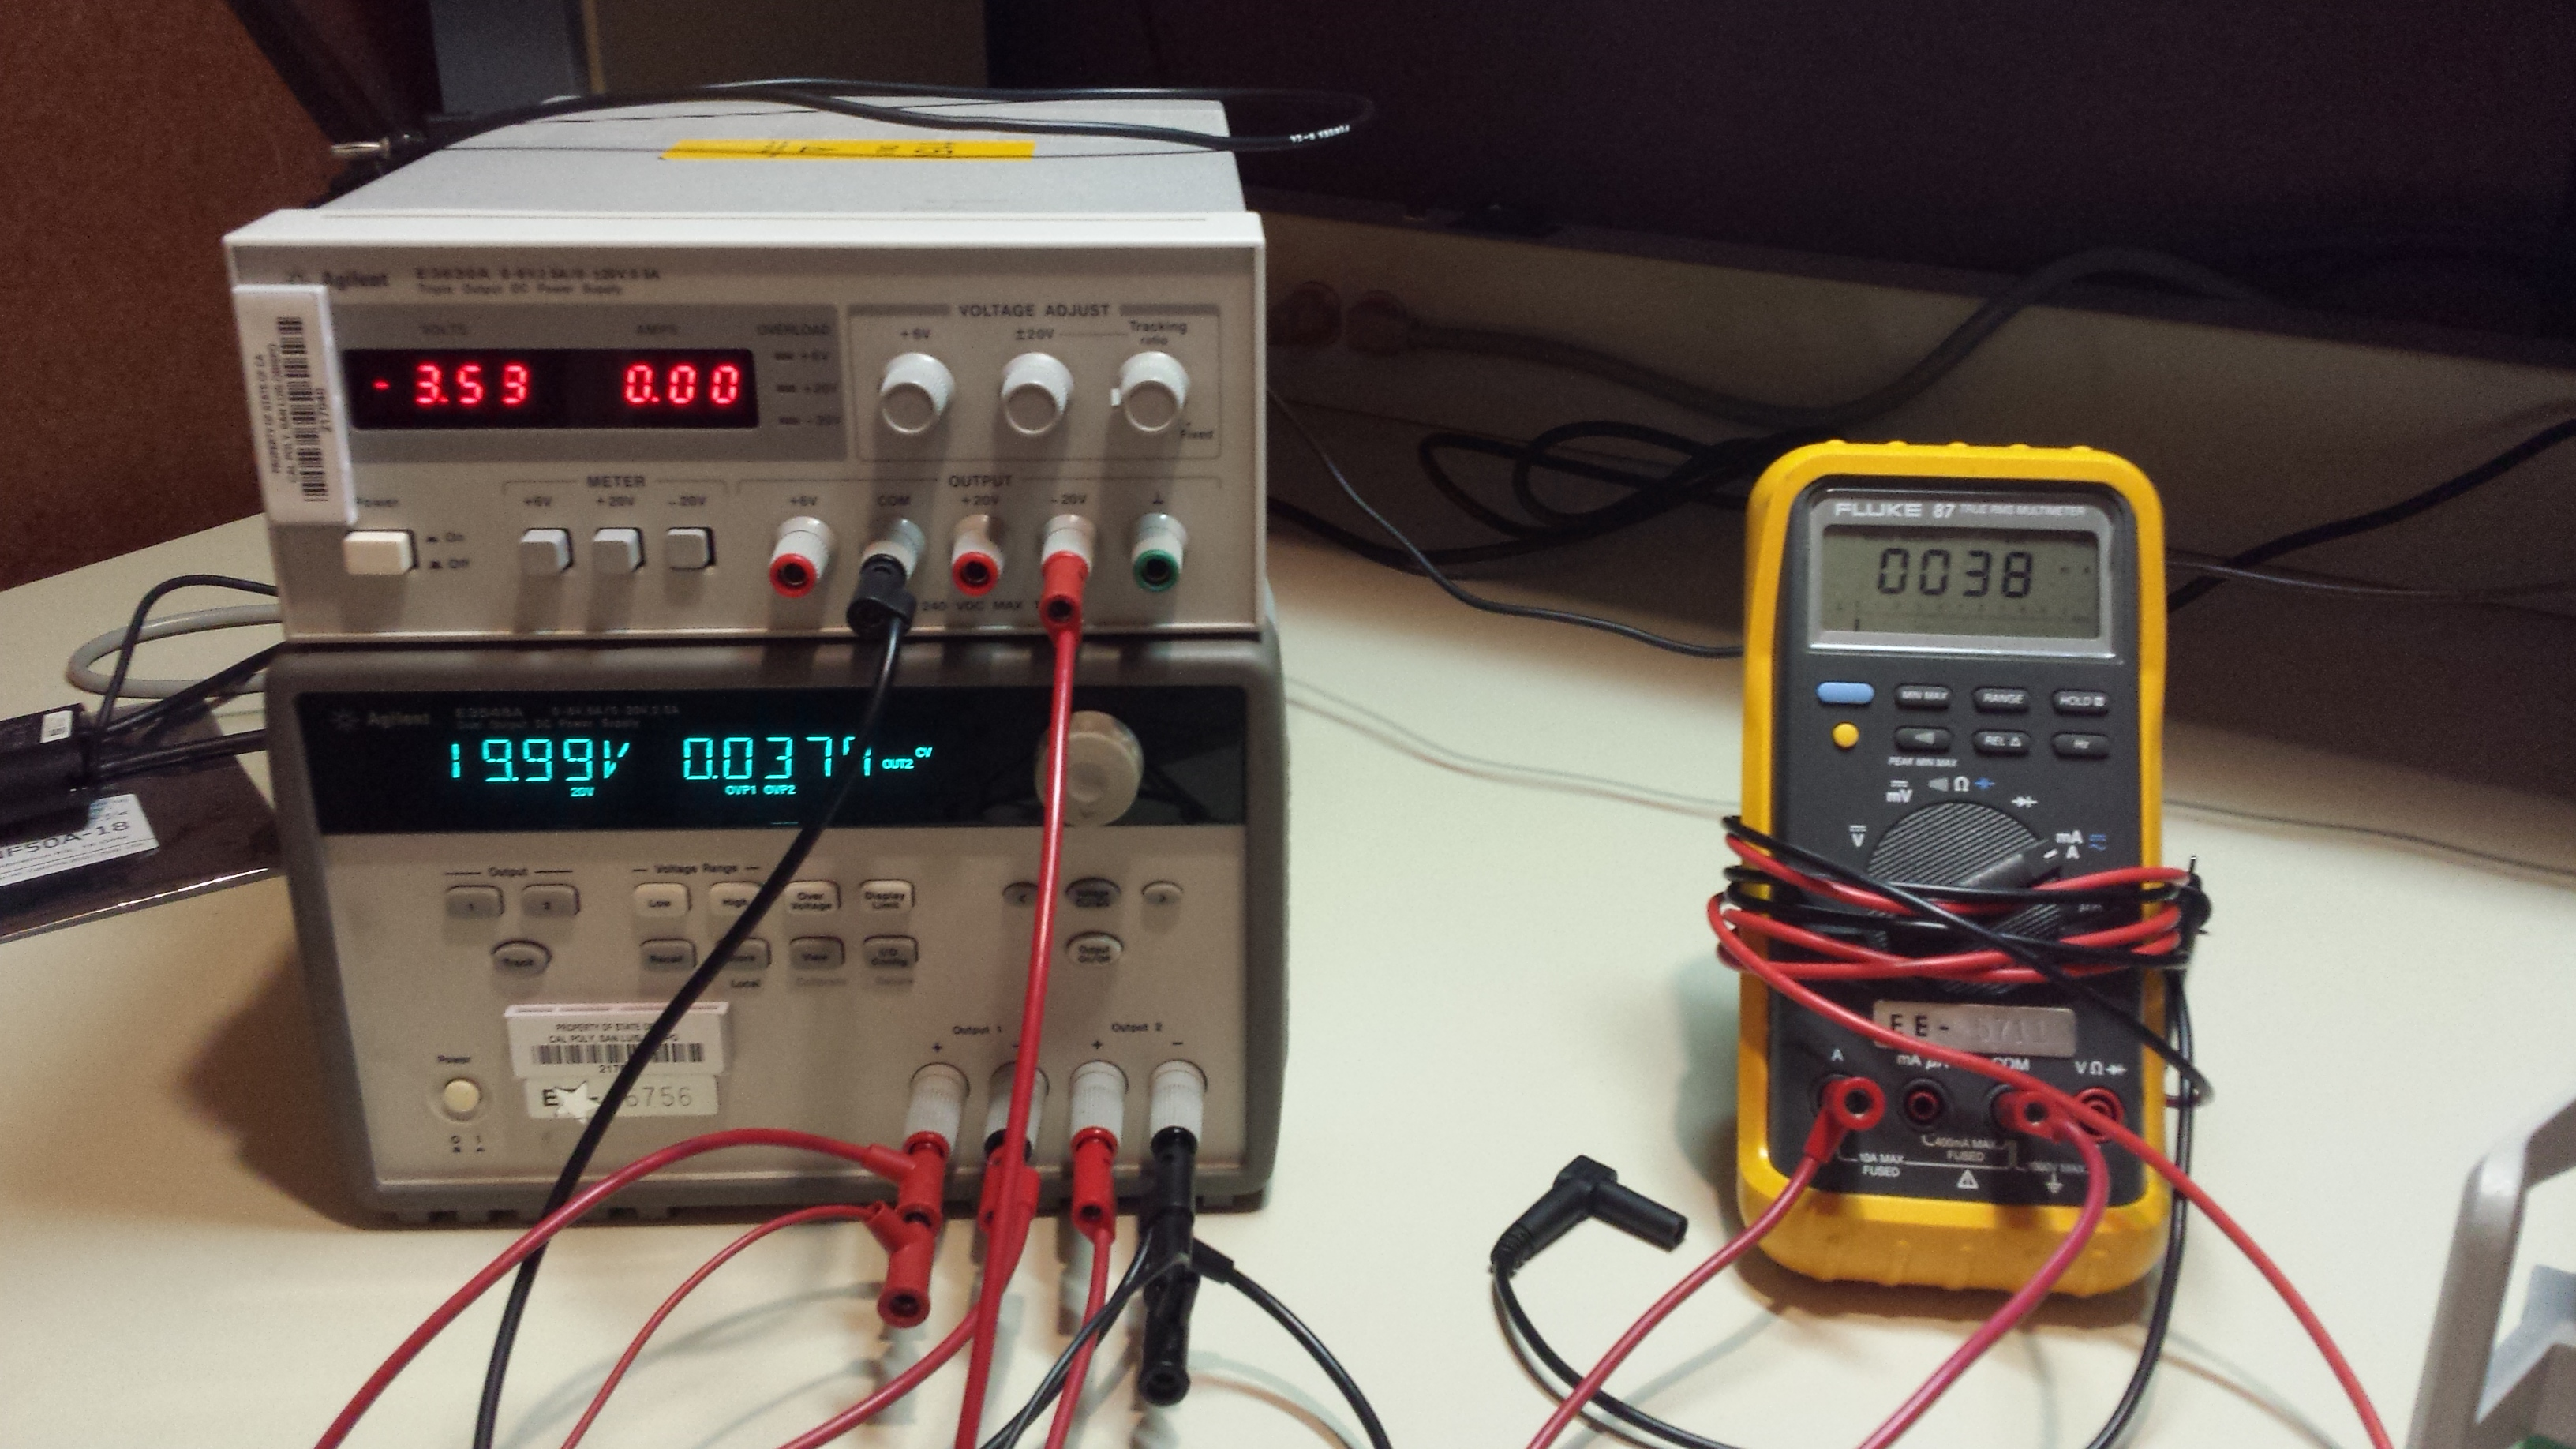
\includegraphics[width=5in,height=5in,keepaspectratio]{figures/test/test_setup}\\
  \caption{Photo of Test Setup}
  \label{fig:test_setup}
\end{figure}

  %\vspace*{\floatsep}
\begin{figure}
  \centering
  % Requires \usepackage{graphicx}
  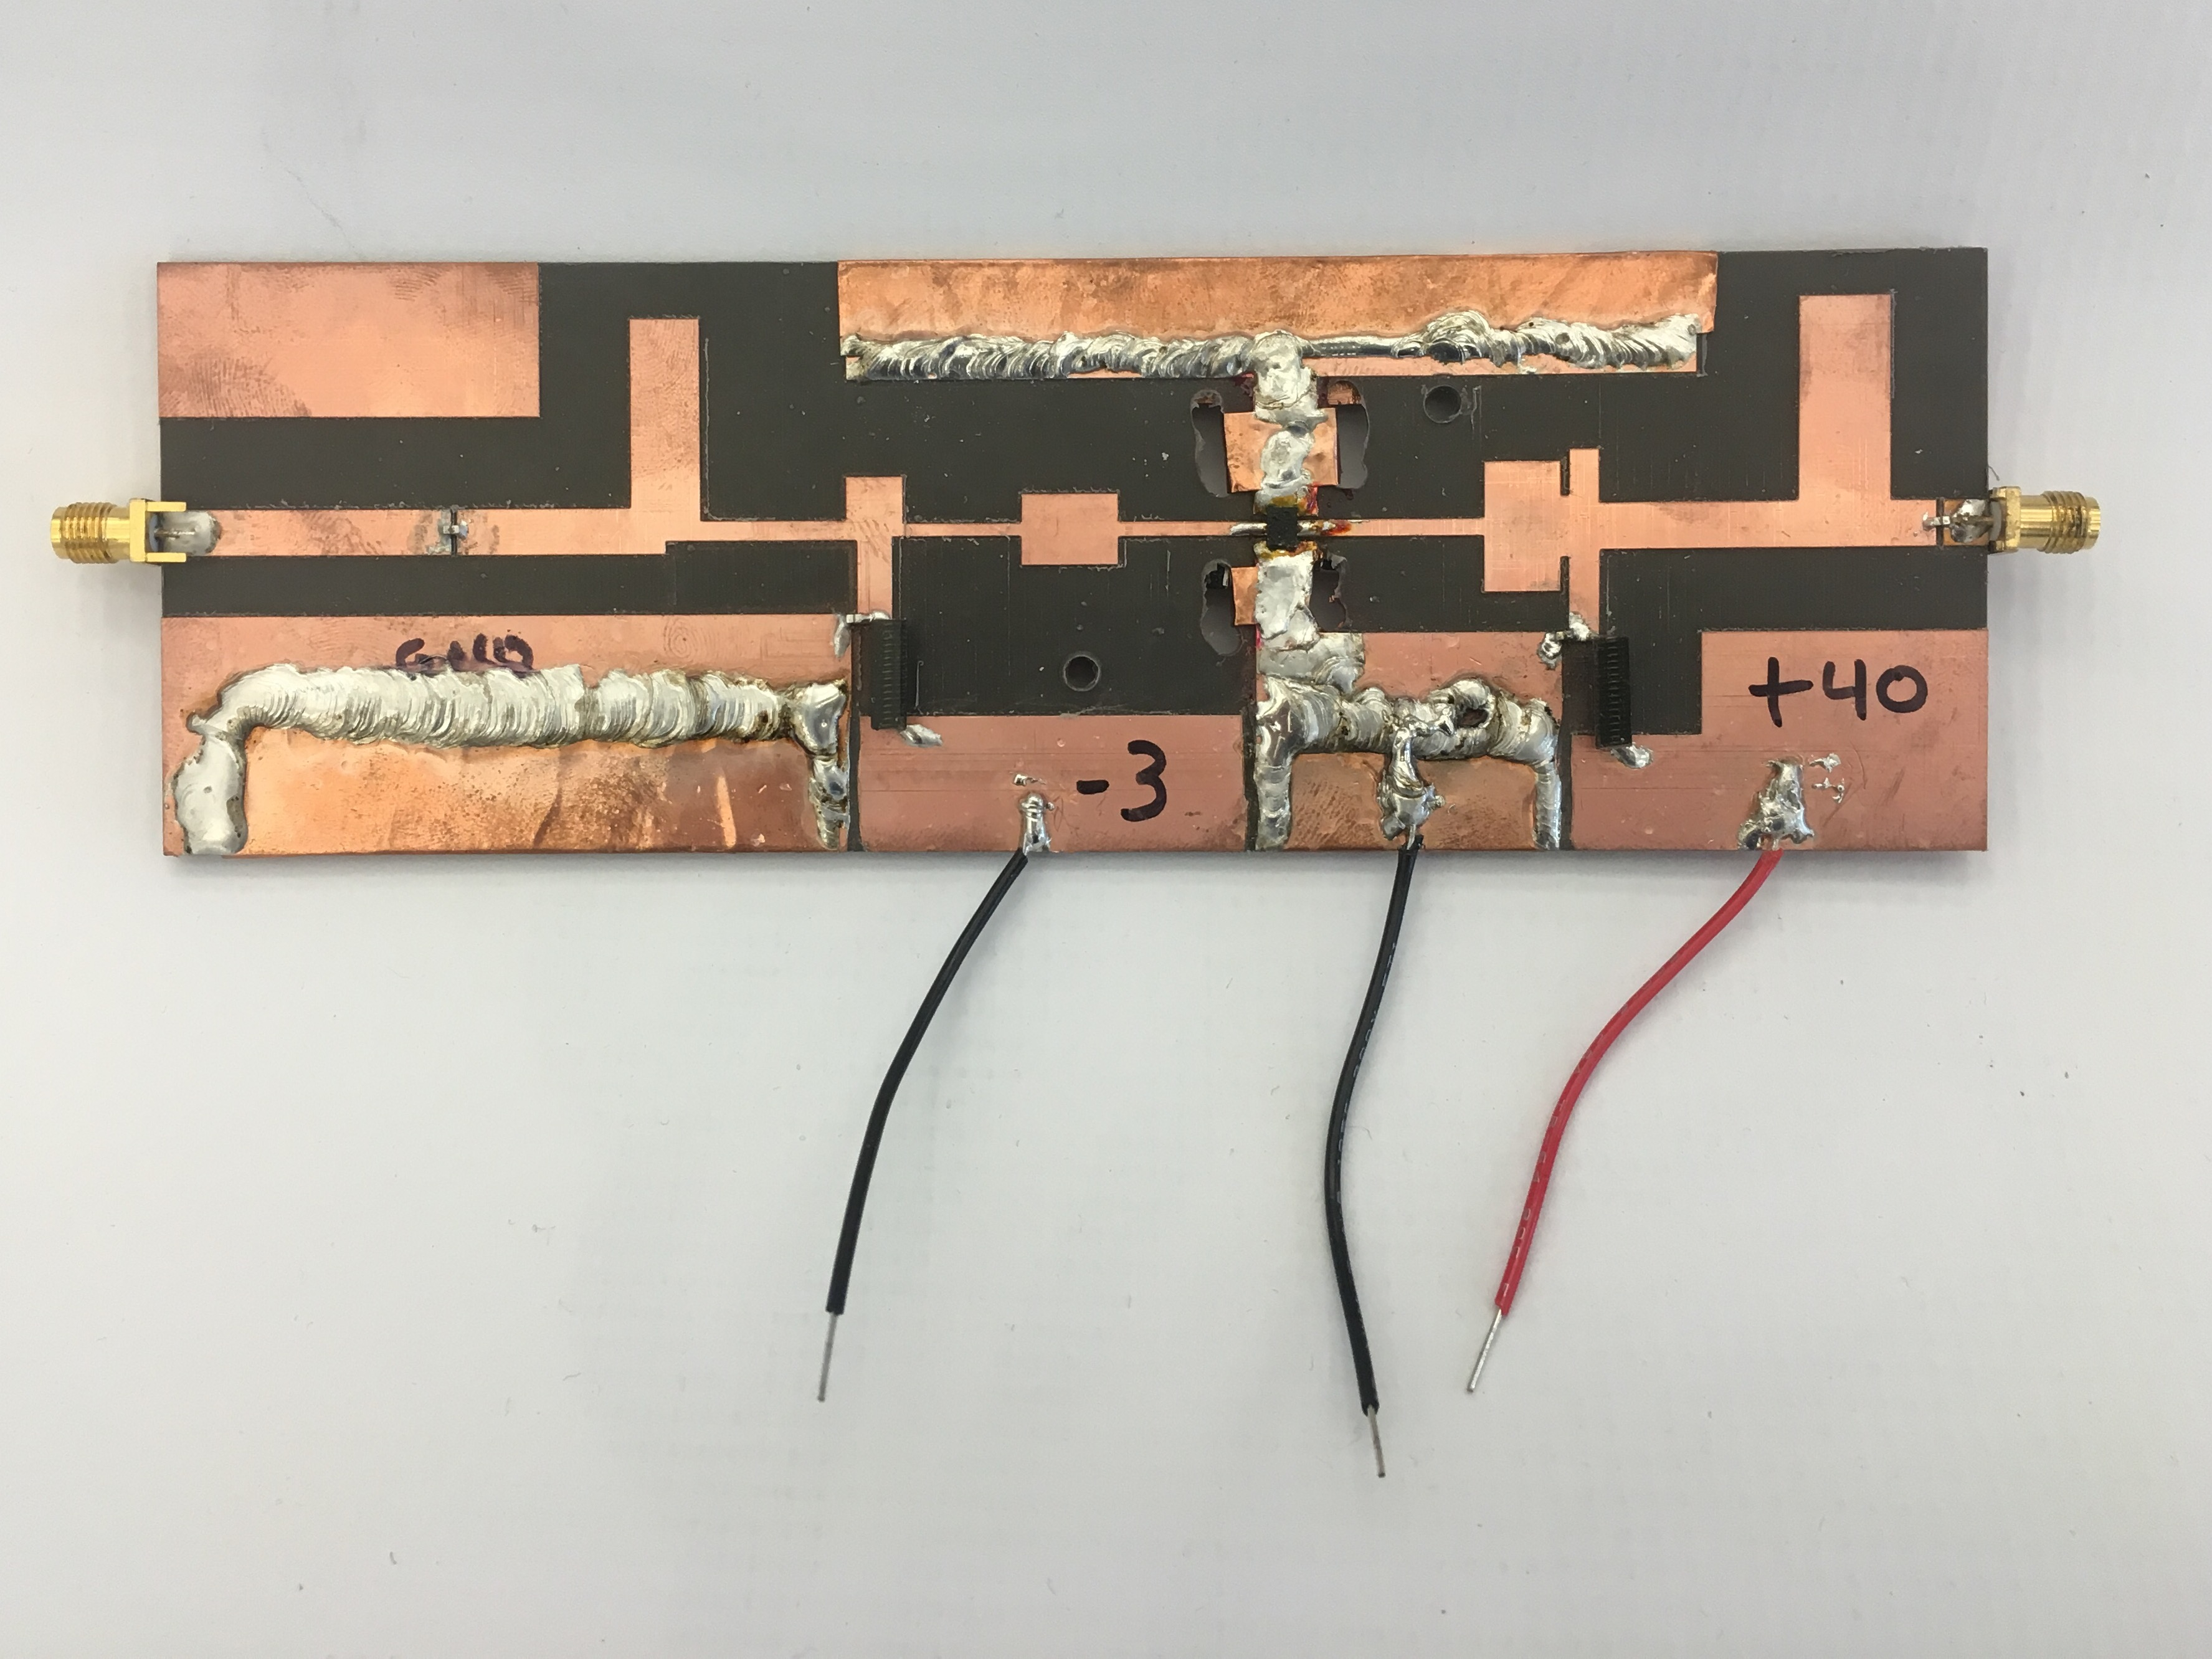
\includegraphics[width=5in,height=5in,keepaspectratio]{figures/test/old_amp}\\
  \caption{Photo of Previous Version of Amplifier}
  \label{fig:old_amp}
\end{figure}
